\section{Auswertung}
\label{sec:Auswertung}
\subsection{Berechnung der Aktivierungsenergie $W$}
Zu Beginn wird aus dem gemessenen Strom $i$ die Stromdichte $j$ berechnet,
indem der Strom durch die
Kreisfläche $A$ geteilt wird. Die im Experiment verwendete Probe besitzt einen
Durchmesser $d =\SI{3}{\milli\meter}$ \cite{V48}, sodass die Stromdichte
durch
\begin{equation}
  j = \frac{i}{A} = \frac{i}{\pi \, \cdot \, \left( \frac{d}{2}\right)^2}
\end{equation}
berechnet werden kann.
\subsubsection{Korrektur des Untergrundes}
% Zum einen kann aus der Steigung von
% \begin{equation}
%   \ln{\left(\frac{\int_T^{T^{*}} \: i(T') \, dT'}{i(T) \: \text{const}} \right)}
%   \label{eqn:lnint}
% \end{equation}
% gegen $\sfrac{1}{T}$, wobei für $i(T^{*}) \approx 0$ gilt, die
% Aktivierungsenergie
% bestimmt werden.
% Hierfür wird erst das Integral $\int_T^{T^{*}} \: i(T') \, dT'$ zu bestimmt.
Zu beachten ist, wie in den Abbildungen \ref{fig:rohdaten1} und
\ref{fig:rohdaten2} zu sehen,
den nahezu linear ansteigenden Untergrundeffekt zu berechnen und abzuziehen.
Aus diesem Grund werden jeweils einige Werte vor und nach dem ersten Peak
ausgewählt und
eine lineare Ausgleichsgerade durch diese gezogen.
Die entsprechenden Werte sind in den Tabellen \ref{tab:1} und Tabelle
\ref{tab:2} zu sehen.
\begin{figure}[H]
\centering
\begin{subfigure}{0.49\textwidth}
\centering
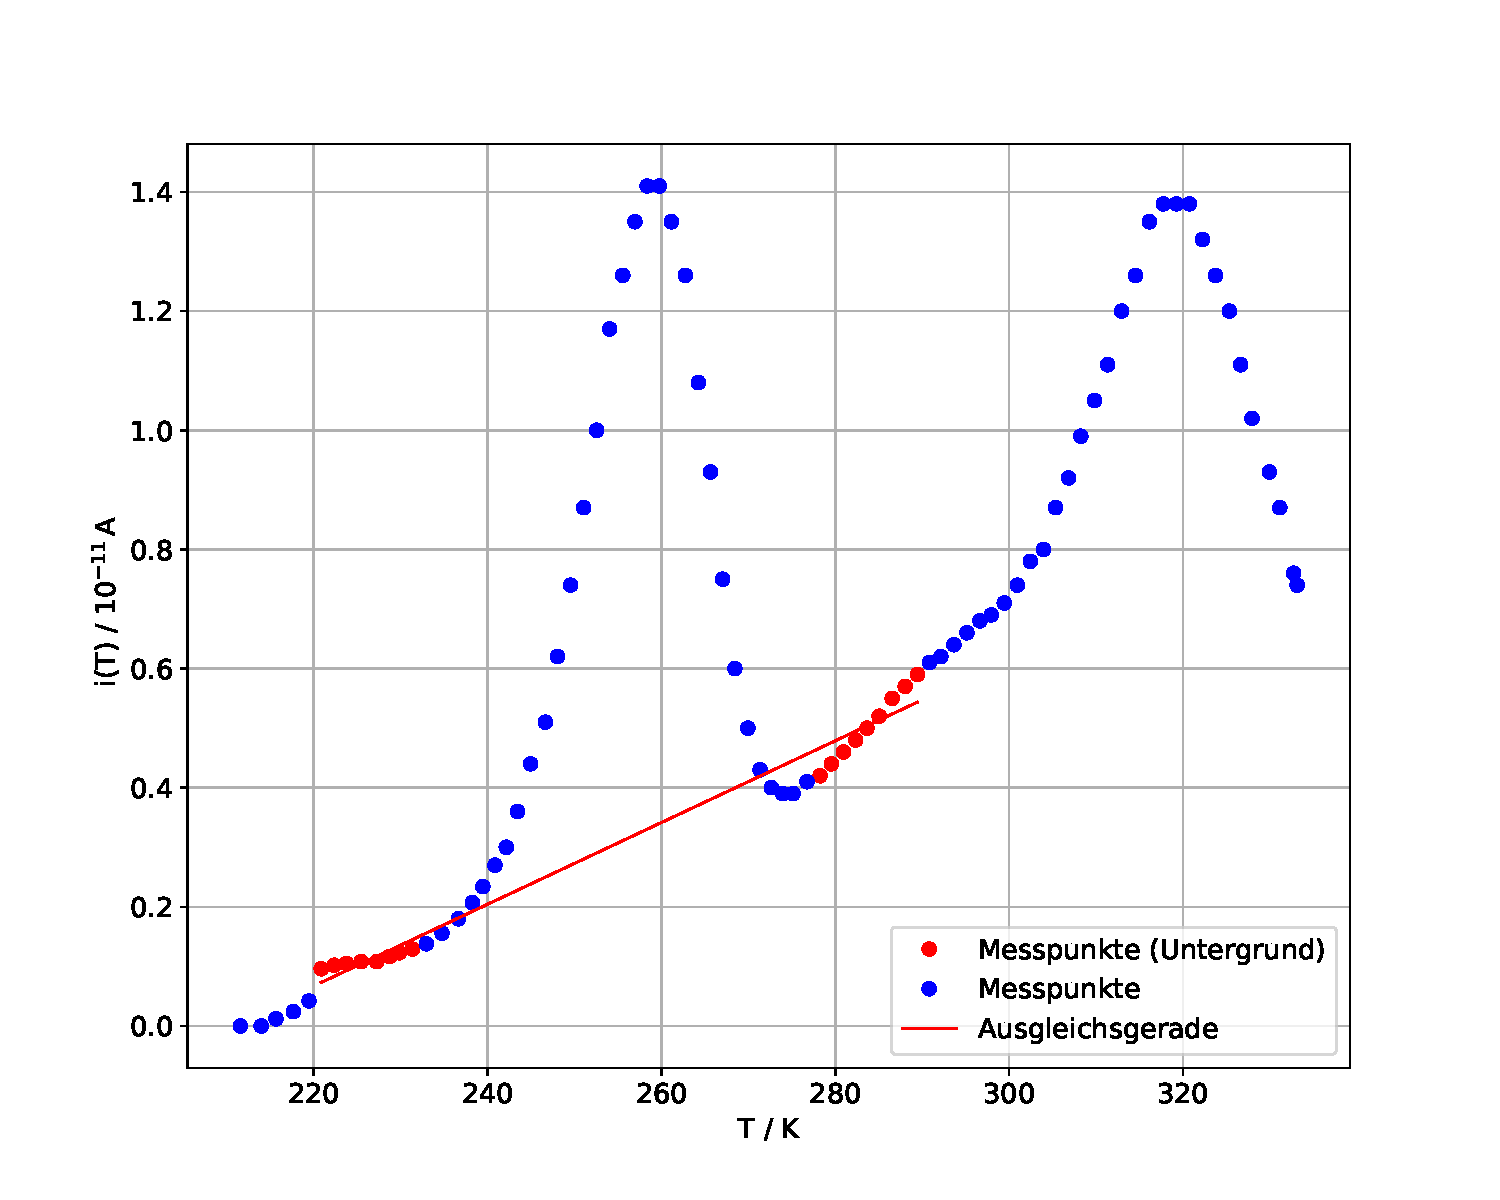
\includegraphics[width=8cm]{Messdaten_1.pdf}
\caption{Stromverlauf mit einer Heizrate $\approx \SI{1.5}{\kelvin\per\minute}$}
\label{fig:rohdaten1}
\end{subfigure}
\begin{subfigure}{0.49\textwidth}
\centering
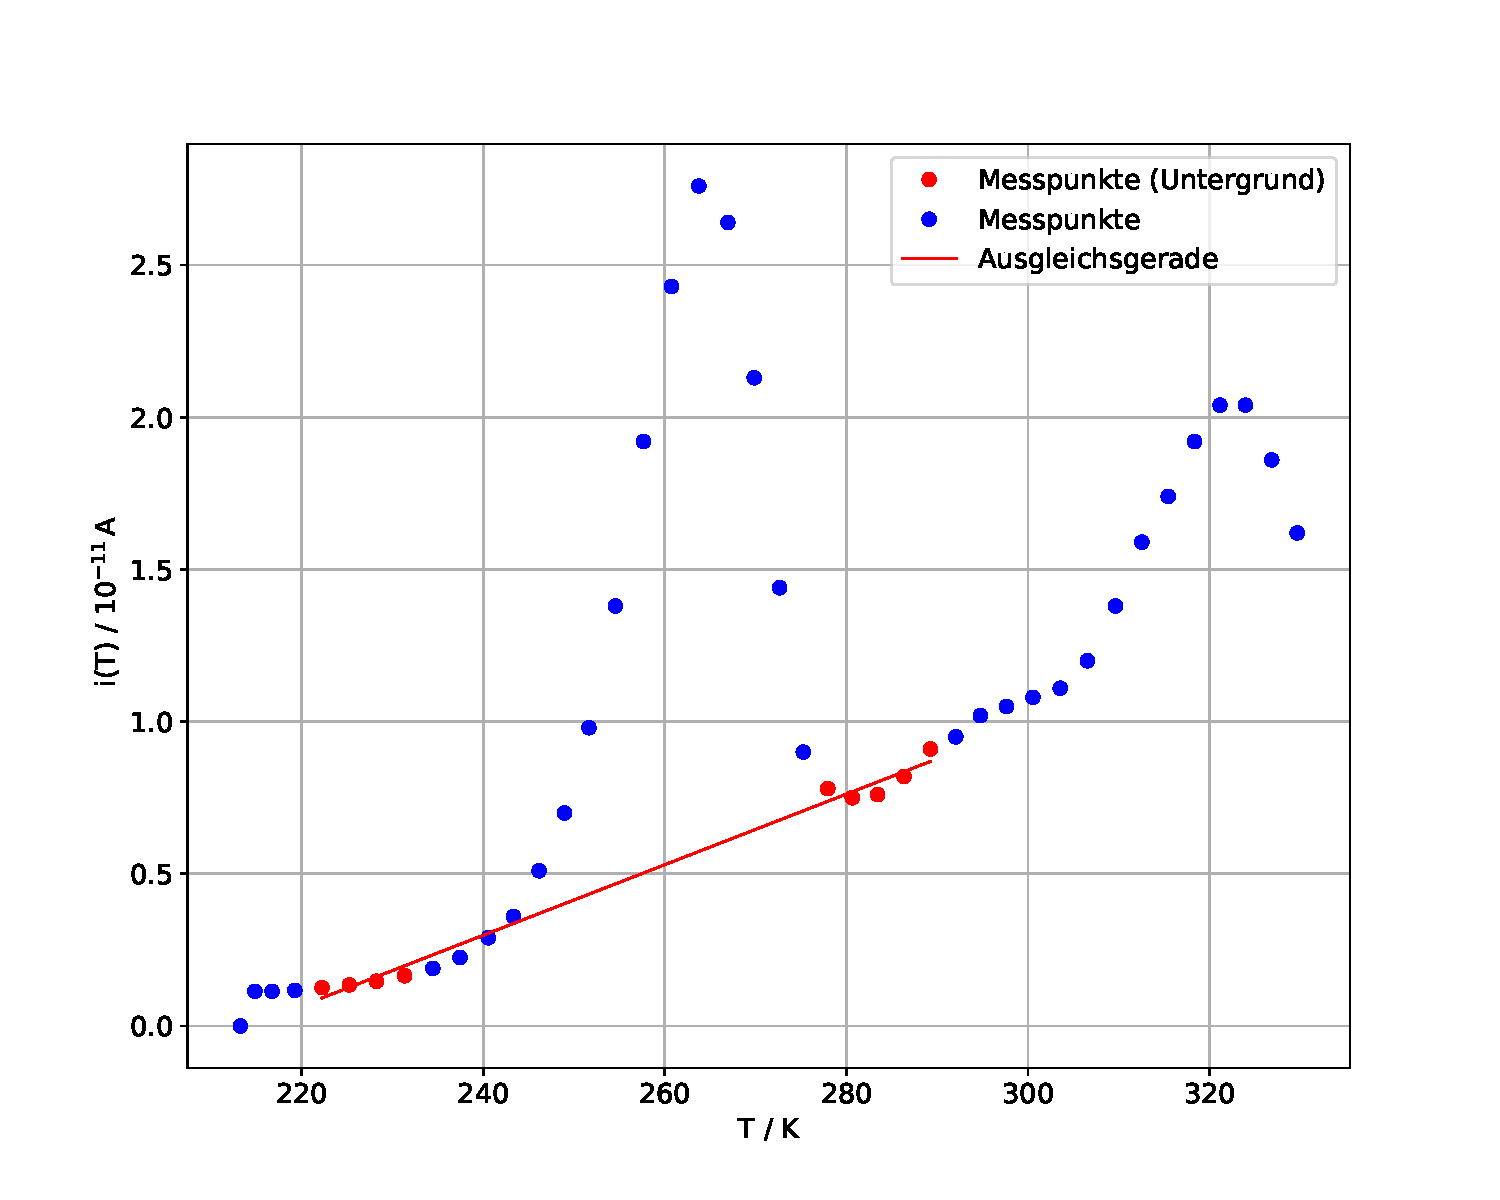
\includegraphics[width=8cm]{Messdaten_2.pdf}
\caption{Stromverlauf mit einer Heizrate $\approx \SI{3.0}{\kelvin\per\minute}$}
\label{fig:rohdaten2}
\end{subfigure}
\caption{Temperaturabhängiger Verlauf des Depolarisationsstroms }
\label{abb:rohdaten}
\end{figure}
Für den Depolarisationsstrom mit einer Heizrate von
$\SI{1.5}{\kelvin\per\minute}$ kann die Ausgleichsgerade
($y(x) = ax + b$)
des Untergrundeffekt durch die Parameter
\begin{align*}
  a_\text{Ausgleich} =& \SI{6.9(2)e-14}{\ampere\per\kelvin}\\
  b_\text{Ausgleich} =& \SI{-1.44(6)e-11}{\ampere}
\end{align*}
bzw. für eine Heizrate von etwa $\SI{3.0}{\kelvin\per\minute}$ durch
\begin{align*}
  a_\text{Ausgleich} =& \SI{1.16(4)e-13}{\ampere\per\kelvin} \\
  b_\text{Ausgleich} =& \SI{-2.5(1)e-11}{\ampere}
\end{align*}
beschrieben werden. Die beiden Geraden sind in den jeweiligen Abbildungen
eingezeichnet.
\subsection{Berechnung von $W$ aus dem gesamten Kurvenverlauf}

Anschließend kann das Integral berechnet werden und in die Formel
\ref{eqn:11}
eingesetzt werden.
Für die Berechnung des Integrals wird jeweils zwischen zwei Messpunkten
eine Gerade der Form
\begin{equation*}
  a_\text{Anstieg} \cdot T + b_\text{Anstieg}
\end{equation*}
gezogen und
die Fläche zwischen dieser Geraden und der Ausgleichsgeraden für die
Hintergrundeffekte berechnet.
Es wird somit jeweils zwischen zwei Messpunkten das Integral
\begin{equation}
  \int^{T_2}_{T_1} \left(a_\text{Anstieg} \cdot T' + b_\text{Anstieg}
  -  a_\text{Ausgleich} \cdot T' -  b_\text{Ausgleich} \right) dT'
  \label{eqn:int}
\end{equation}
ermittelt. Durch Aufsummieren der Teilintegrale bis zum jeweiligen Punkt, wird
das Gesamtintegral $i_\text{Int}$ berechnet (Tabelle \ref{tab:3} und \ref{tab:4}).
In Abbildung \ref{fig:int_1} und \ref{fig:int_2} sind $ln(\sfrac{i_\text{Int}}{i(T_2)})$  gegen $\sfrac{1}{T}$
aufgetragen und eine Ausgleichsgerade durch
die berechneten Wertepaare gelegt worden.
\begin{figure}[H]
\centering
\begin{subfigure}{0.49\textwidth}
\centering
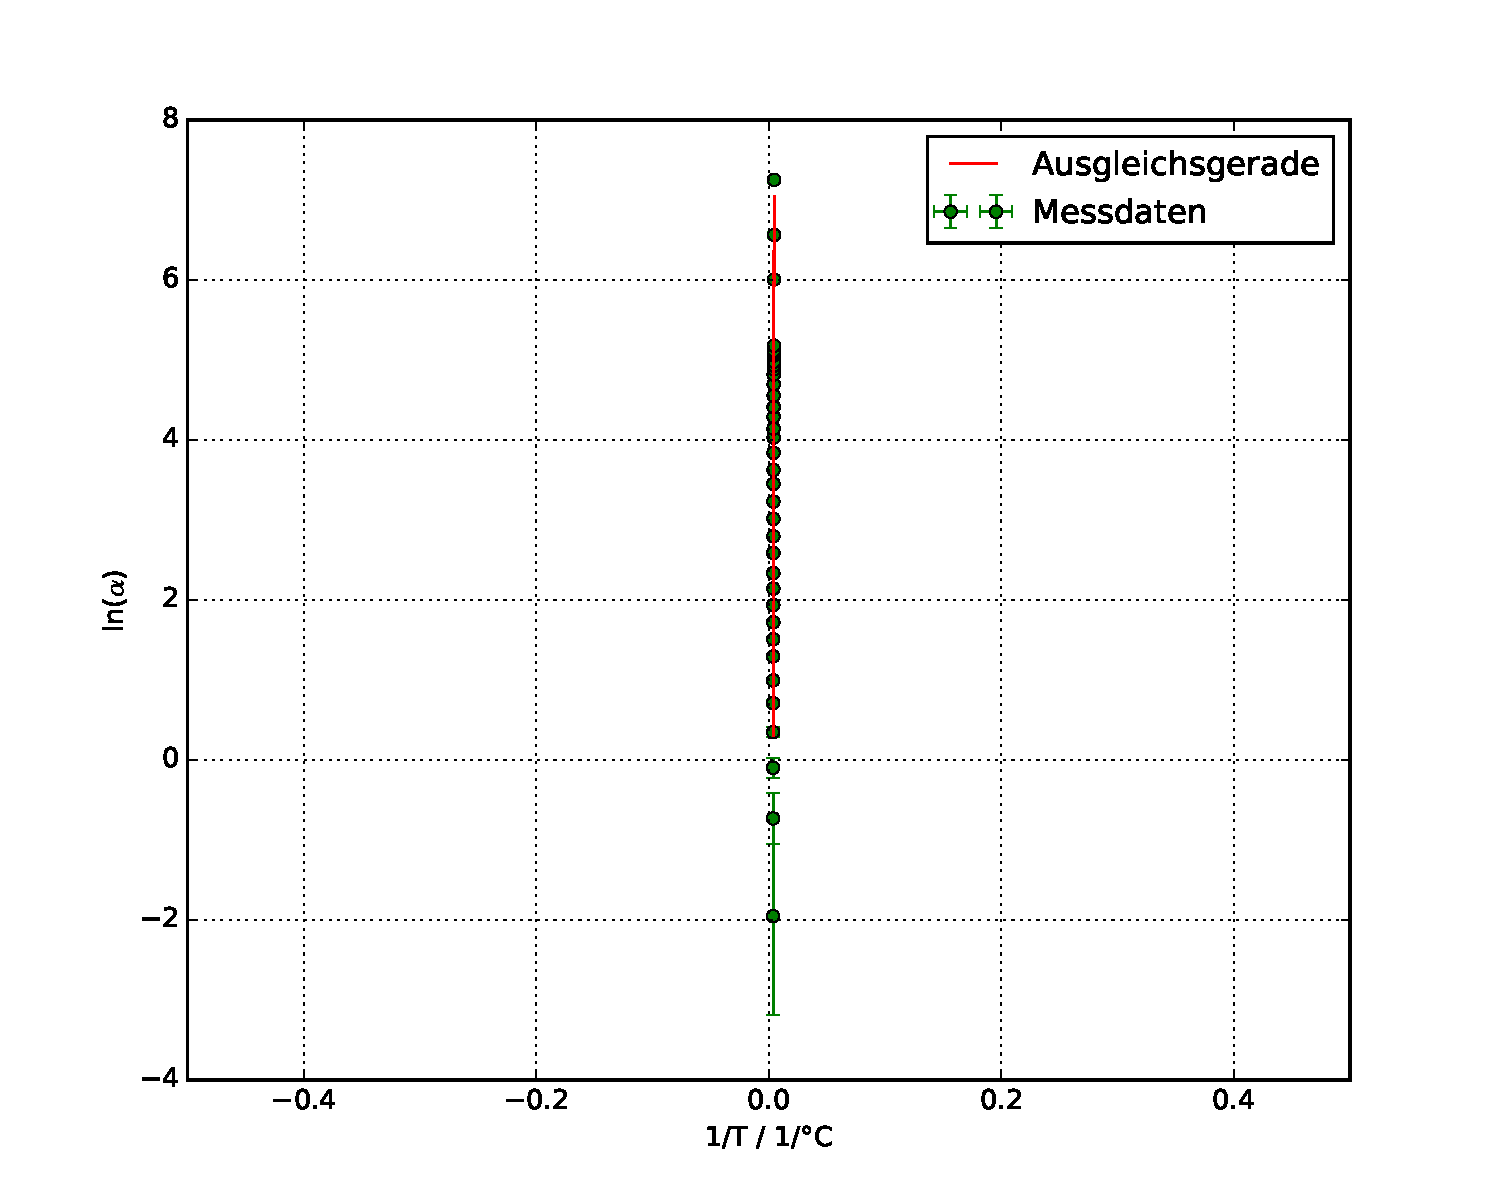
\includegraphics[width=8.0cm]{int_1.pdf}
\caption{Bestimmung der Aktivierungsenergie mit einer Heizrate
$\approx \SI{1.5}{\kelvin\per\minute}$}
\label{fig:int_1}
\end{subfigure}
\begin{subfigure}{0.49\textwidth}
\centering
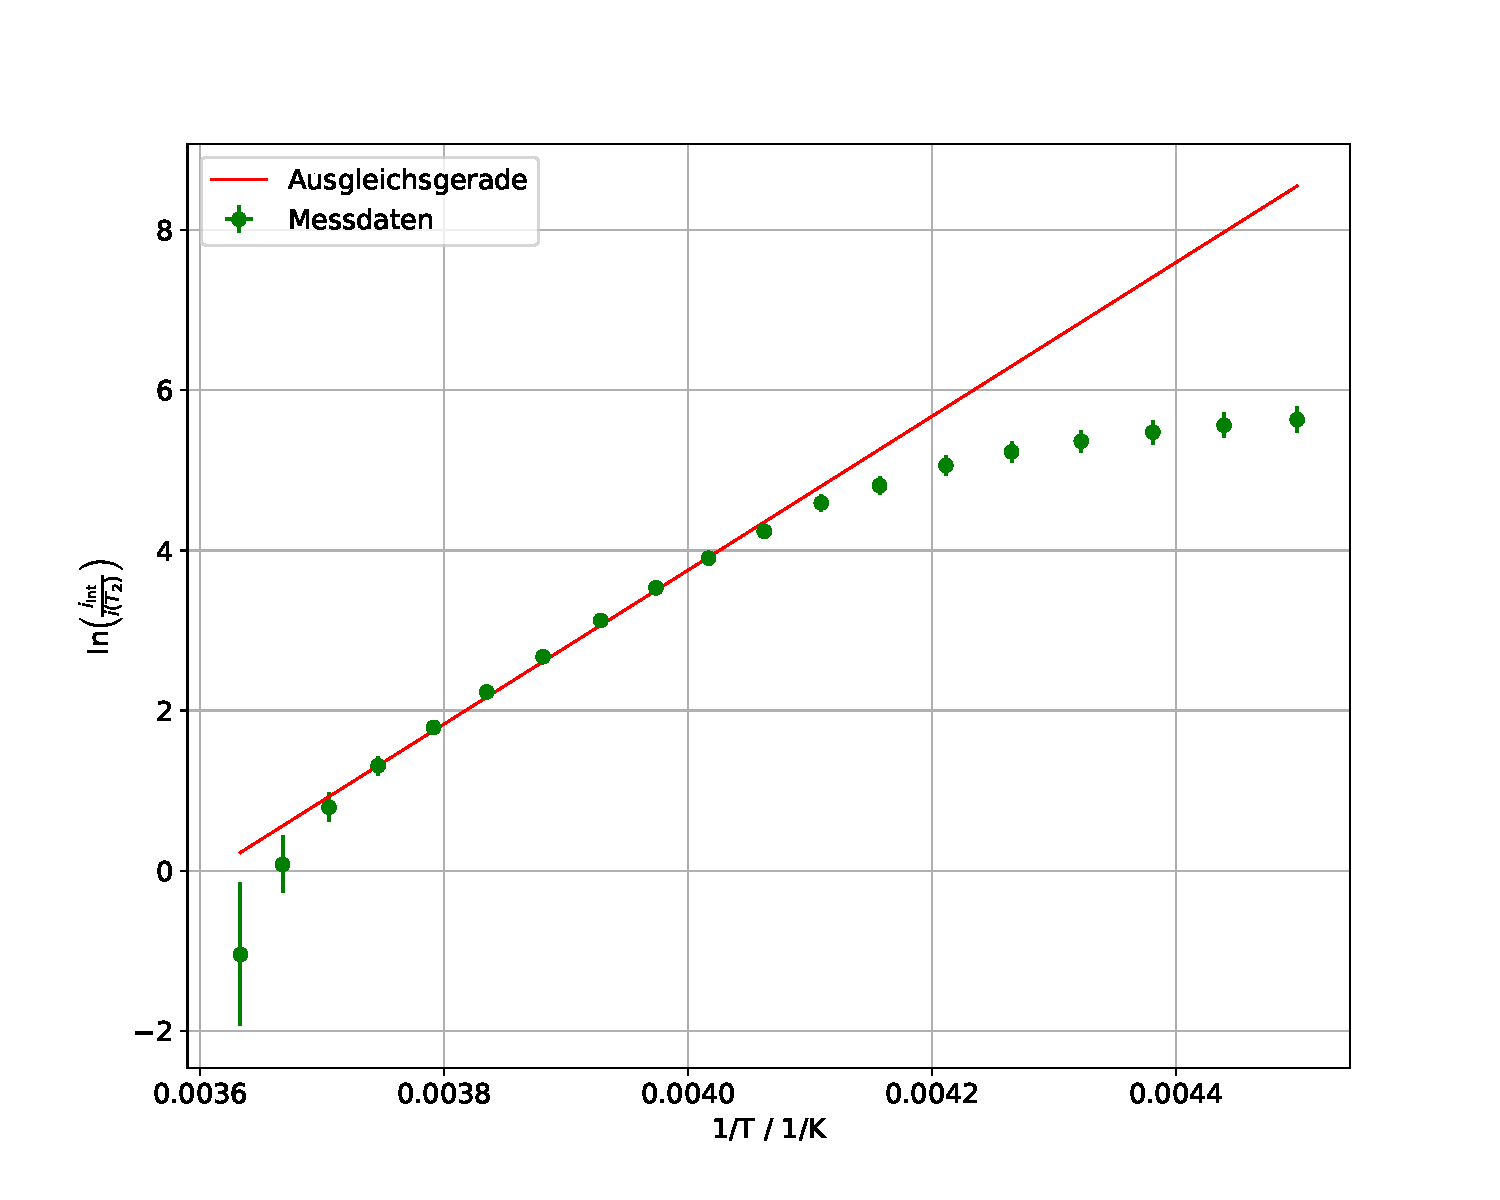
\includegraphics[width=8.0cm]{int_2.pdf}
\caption{Bestimmung der Aktivierungsenergie mit einer Heizrate
$\approx \SI{3.0}{\kelvin\per\minute}$}
\label{fig:int_2}
\end{subfigure}
\caption{Bestimmung der Aktivierungsenergie}
\label{abb:int_ges}
\end{figure}
Es ergibt sich eine Steigung und Y-Achsenabschnitt von
\begin{align*}
  a_{\text{int}_1} =& \SI{8700(200)}{\kelvin} \\
  %\Delta a_W =& \SI{400}{\kelvin} \\
  b_{\text{int}_1} =& \num{-32(1)}
\end{align*}
für die Heizrate von $\SI{1.5}{\kelvin\per\minute}$
und für die Heizrate von $\SI{3.0}{\kelvin\per\minute}$ ist die
Steigung bzw. Y-Achsenabschnitt von
\begin{align*}
  a_{\text{int}_2} =& \SI{9600(200)}{\kelvin} \\
  %\Delta a_W =& \SI{400}{\kelvin} \\
  b_{\text{int}_2} =& \num{-34(1)}.
\end{align*}

% Da der gemessene Depolarisationsstroms nach Abzug des Untergrundeffekt und
% resultierend das Integral über den Depolarisationsstroms sowie
% die Parameter  der durch das Integral gezogene Ausgleichsgerade einen Fehler
% besitzt, wird für den Fehler der Steigung angewendet.
Da die Ausgleichsparameter $a_\text{Ausgleich}$ und $b_\text{Ausgleich}$ fehlerbelastet
sind, ist auch das Integral über den Depolarisationsstroms fehlerbelastet.
Der Fehler des Integrals (Formel \ref{eqn:int}) errechnet sich aus
\begin{equation}
\Delta I =  \sqrt{\left(\frac{T^2 \, \Delta a_\text{Ausgleich}}{2}\right)^2 +
  (\Delta b_\text{Ausgleich} T)^2}.
\end{equation}
% Daher kann der Fehler der Steigung der Ausgleichsgerade für die Bestimung
% der Aktivierungsenergie
% durch die Formel
% \begin{equation}
%   \Delta a_W = \sqrt{(\Delta I \, \cdot a)^2 \: + \: (\Delta a_\text{steigung}
%   \, \cdot \, I)^2}
% \end{equation}
% ermittelt werden.
Durch Umstellen des Verhältnis (Formel \ref{eqn:strom2})
\begin{equation}
  a = \frac{W}{\text{k}_\text{B}} \iff W = a \cdot \text{k}_\text{B}
  \label{eqn:verhaltnis}
\end{equation}
kann die Aktivierungsenergie $W$ zu
\begin{equation*}
  W_\text{1a} = \SI{120(3)e-21}{\joule} = \SI{0.75(2)}{\electronvolt}
\end{equation*}
für die Messreihe mit Heizrate $b \approx \SI{1.5}{\kelvin\per\minute}$
berechnet werden.
Analog kann dies für die Messreihe mit $b \approx \SI{3.0}{\kelvin\per\minute}$
ermittelt werden.
Es ergibt sich eine Aktivierungsenergie von
\begin{equation*}
W_\text{2a} =  \SI{133(3)e-21}{\joule} = \SI{0.83(2)}{\electronvolt}.
\end{equation*}
\subsubsection{Berechnung der Aktivierungsenergie $W$ über linearen Anstieg}
Eine andere Methode zur Bestimmung der Aktivierungsenergie $W$ ist es $\ln(j)$
gegen $\sfrac{1}{T}$ im Anfagsbereich der Depolarisationskurve
aufzutragen und mit Hilfe einer Ausgleichsgerade sowie dem
Verhältnis
\begin{equation}
  a = -\frac{W}{\text{k}_\text{B}} \iff W = -a \cdot \text{k}_\text{B}
\end{equation}
dieses zu berechnen.
Der Zusammenhang wurde in der Theorie in Formel \ref{eqn:stmet1} gezeigt und für
die Berechnung umgestellt.
Grundlage hierfür ist die in Formel \ref{eqn:7} erwähnte Näherung und die daraus
resultierende Annahme (Formel \ref{eqn:stmet1}).
In Abbildung \ref{fig:j_1} und Abbildung \ref{fig:j_2} ist $\ln(j)$
gegen $\sfrac{1}{T}$ gezeigt, während die errechneten Werte in
Tabelle \ref{tab:5} und \ref{tab:6} abgebildet sind.
Im jeweiligen lineare Anstieg des Graphen ist die
erwähnte Ausgleichsgerade eingezeichnet, um aus dessen Parametern die
Aktivierungsenergie zu bestimmen.
\begin{figure}[H]
\centering
\begin{subfigure}{0.49\textwidth}
\centering
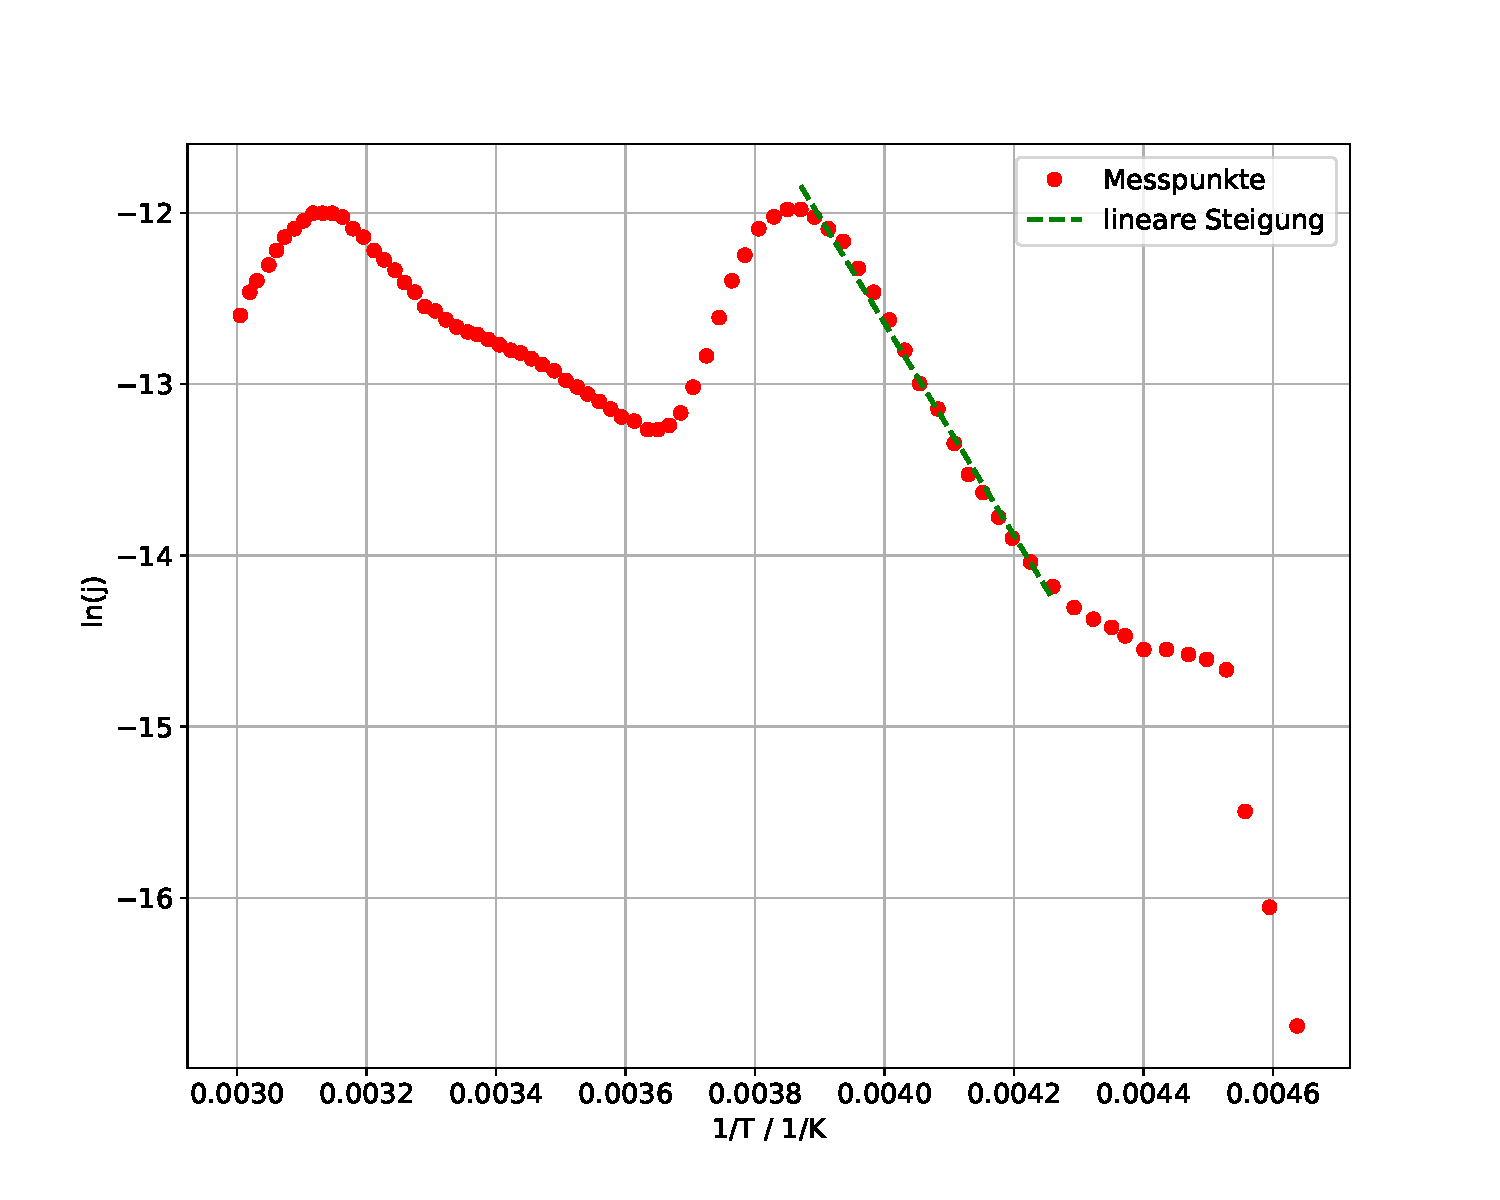
\includegraphics[width=8.0cm]{Messdaten_1_lnj.pdf}
\caption{Bestimmung der Aktivierungsenergie mit einer Heizrate
$\approx \SI{1.5}{\kelvin\per\minute}$}
\label{fig:j_1}
\end{subfigure}
\begin{subfigure}{0.49\textwidth}
\centering
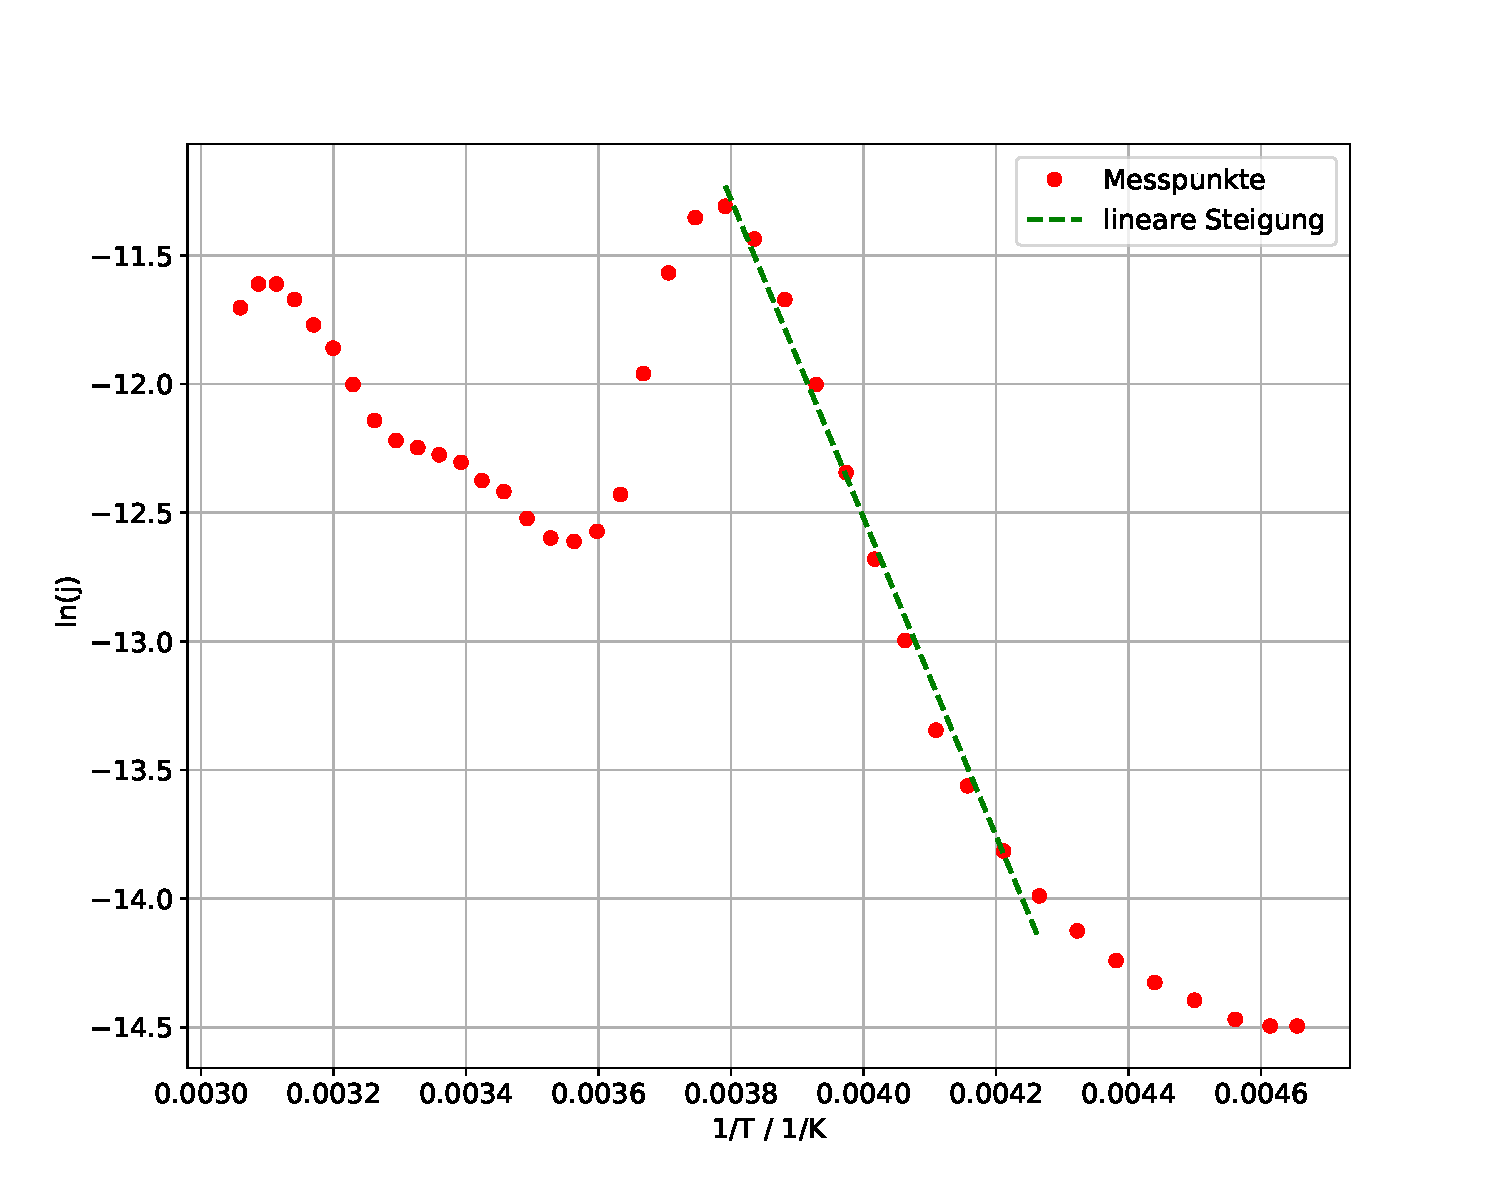
\includegraphics[width=8.0cm]{Messdaten_2_lnj.pdf}
\caption{Bestimmung der Aktivierungsenergie mit einer Heizrate
$\approx \SI{3.0}{\kelvin\per\minute}$}
\label{fig:j_2}
\end{subfigure}
\caption{Bestimmung der Aktivierungsenergie durch linearen Anstieg}
\label{abb:j_ges}
\end{figure}
Für die Messreihe mit der niedrigeren Heizrate ergeben sich die Parameter
\begin{align*}
  a =& \SI{-6200(100)}{\kelvin} \\
  b =& \num{12.1(5)}
\end{align*}
und resultierend eine Aktivierungsenergie von
\begin{equation*}
  W = \SI{85(1)e-21}{\joule} = \SI{0.53(1)}{\electronvolt}.
\end{equation*}
Bei analogem Vorgehen für die andere Messung lassen sich die Parameter
\begin{align*}
  a =& \SI{-6200(200)}{\kelvin} \\
  b =& \num{12.2(9)e-21}
\end{align*}
und eine Aktivierungsenergie $W$ von
\begin{equation*}
  W = \SI{85(3)}{\joule} = \SI{0.53(2)}{\electronvolt}
\end{equation*}
ermitteln.
\subsubsection{Mittelung der Aktivierungsenergie $W$}
In den beiden letzten beiden Unterkapiteln wurden die folgenden Werte für die
Aktivierungsenergie $W$ bestimmt: \\
Integralmethode:
\begin{equation*}
  W_\text{1a} = \SI{120(3)e-21}{\joule} \text{ und } W_\text{2a} =
  \SI{133(3)e-21}{\joule}
\end{equation*}
Methode der linearen Steigung:
\begin{equation*}
  W_\text{1b} = \SI{85(1)e-21}{\joule} \text{ und } W_\text{2b} =
  \SI{85(3)e-21}{\joule}
\end{equation*}
Eine Mittelung der Werte einer Messreihe ergibt eine Aktivierungsenergie von
\begin{align*}
  W_1 &= \SI{102(2)e-21}{\joule} = \SI{0.64(1)}{\electronvolt}\\
  & \text{ und } \\
  W_2 &= \SI{109(2)e-21}{\joule} = \SI{0.68(1)}{\electronvolt}
\end{align*}
wobei der Fehler durch die Gauß'sche Fehlerfortpflanzung mit der Formel
\begin{equation}
  \Delta W = \frac{1}{2} \: \sqrt{(\Delta W_a)^2 + (\Delta W_a)^2}
\end{equation}
berechnet wird.
\subsection{Bestimmung der Relaxationszeit}
Um die Relaxationszeit $\tau_0$ zu bestimmen wird Formel \ref{eqn:tau}
verwendet.
Der auftretende Fehler auf $\tau_0$ kann durch
\begin{equation}
  \Delta \tau_0 = \sqrt{
  \left(-\frac{\text{k}_\text{B} \, T_\text{max}^2}{W \, b_\text{heiz}^2} \cdot
  e^{-\frac{W}{\text{k}_\text{B} \, T_\text{max}}} \cdot \Delta b_\text{heiz}
  \right)^2 +
  \left(-\frac{(\text{k}_\text{B} \, T_\text{max} + W) \, T_\text{max}}{W^2 \,
  b_\text{heiz}} \cdot
  e^{-\frac{W}{\text{k}_\text{B} \, T_\text{max}}} \cdot \Delta W \right)^2
  }
  \label{eqn:tau_fehler}
\end{equation}
ermittelt werden. In dieser Formel steht $b_\text{heiz}$ für die Heizrate,
welche im folgenden Unterkapitel für die beiden Messreihen bestimmt wird.
\subsubsection{Bestimmung der Heizrate $b_\text{heiz}$}
Für die Berechnung der durchschnittlichen Heizrate werden die
Temperaturen gegen die Messzeit aufgetragen und eine Ausgleichsgerade angelegt.
In Abbildungen \ref{fig:heiz1} und \ref{fig:heiz2} sind die beiden Messreihen
und deren Ausgleichsgerade abgebildet.
\begin{figure}
  \centering
  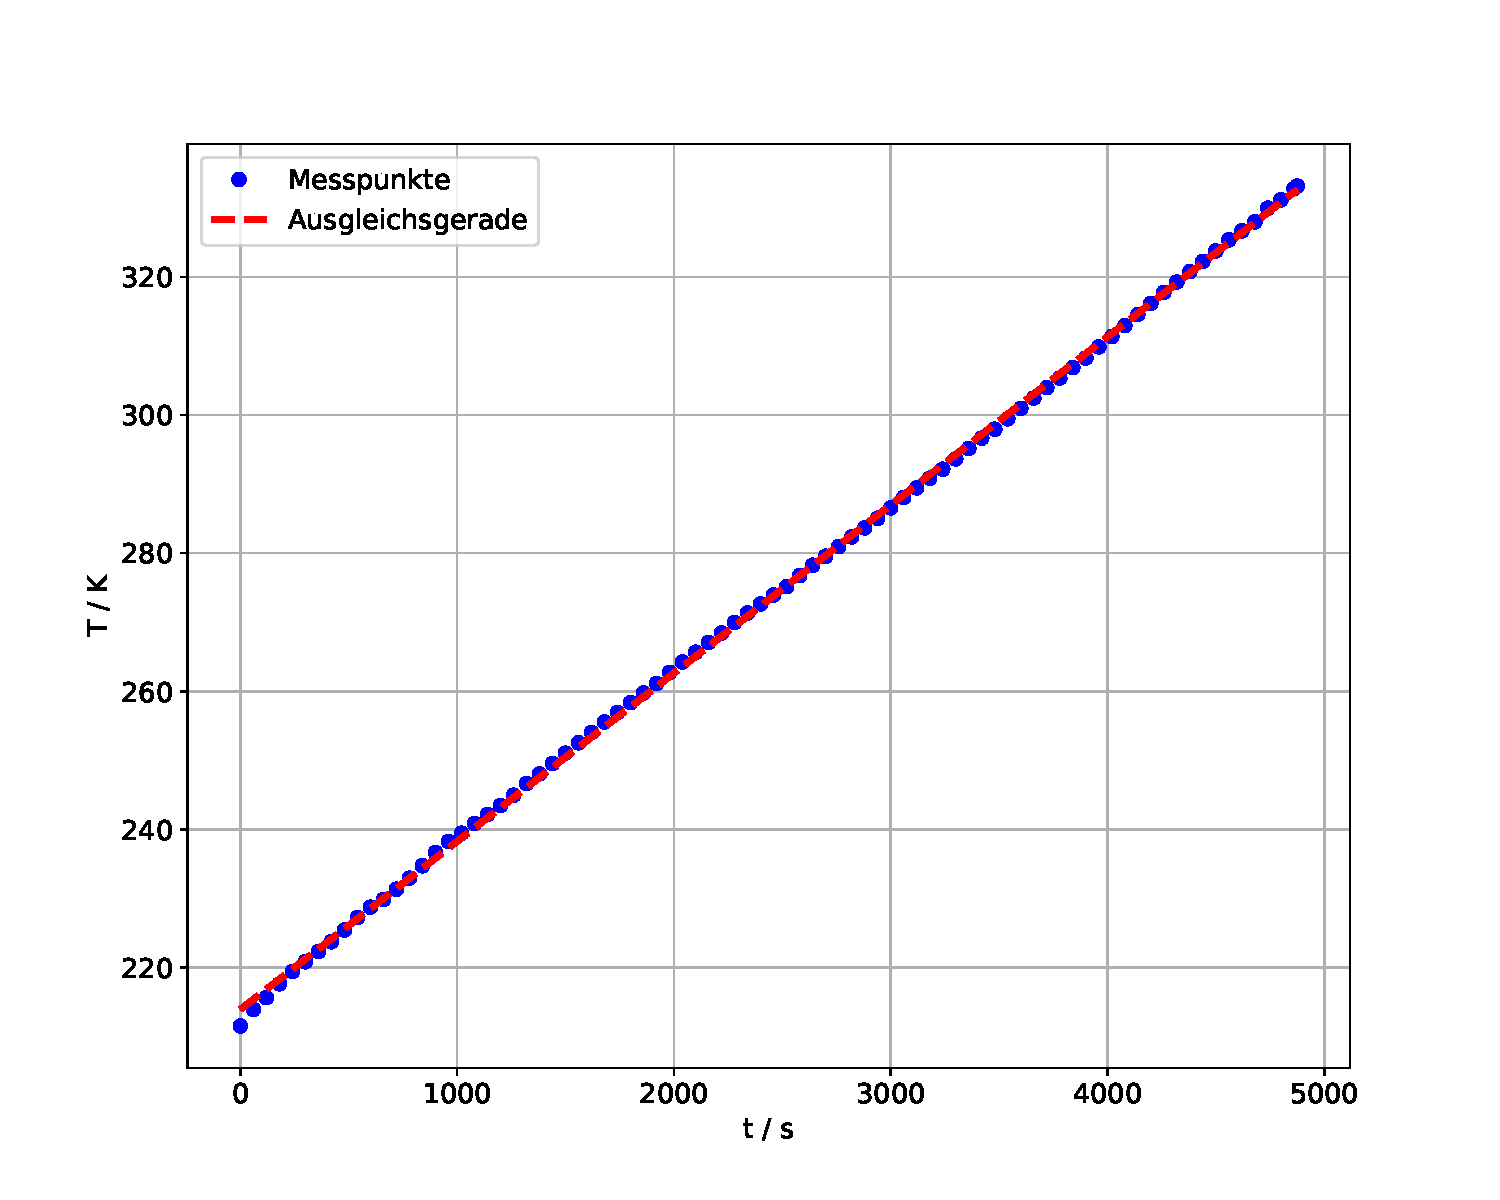
\includegraphics[width=10.0cm]{Messdaten_1_rate.pdf}
  \caption{Berechnung der mittleren Heizrate für die Messung
  mit $b_\text{heiz} \approx \SI{1.5}{\kelvin\per\minute}$}
  \label{fig:heiz1}
\end{figure}
Die Ausgleichsparameter der Geraden der Form $b_\text{heiz} \cdot T + c$
sind:
\begin{align*}
  b_\text{heiz} =& \SI{2434(4)e-05}{\kelvin\per\second} = \SI{1.460(2)}{\kelvin\per\minute}\\
  c = & \SI{213.9(1)}{\kelvin}
\end{align*}
\begin{figure}
  \centering
  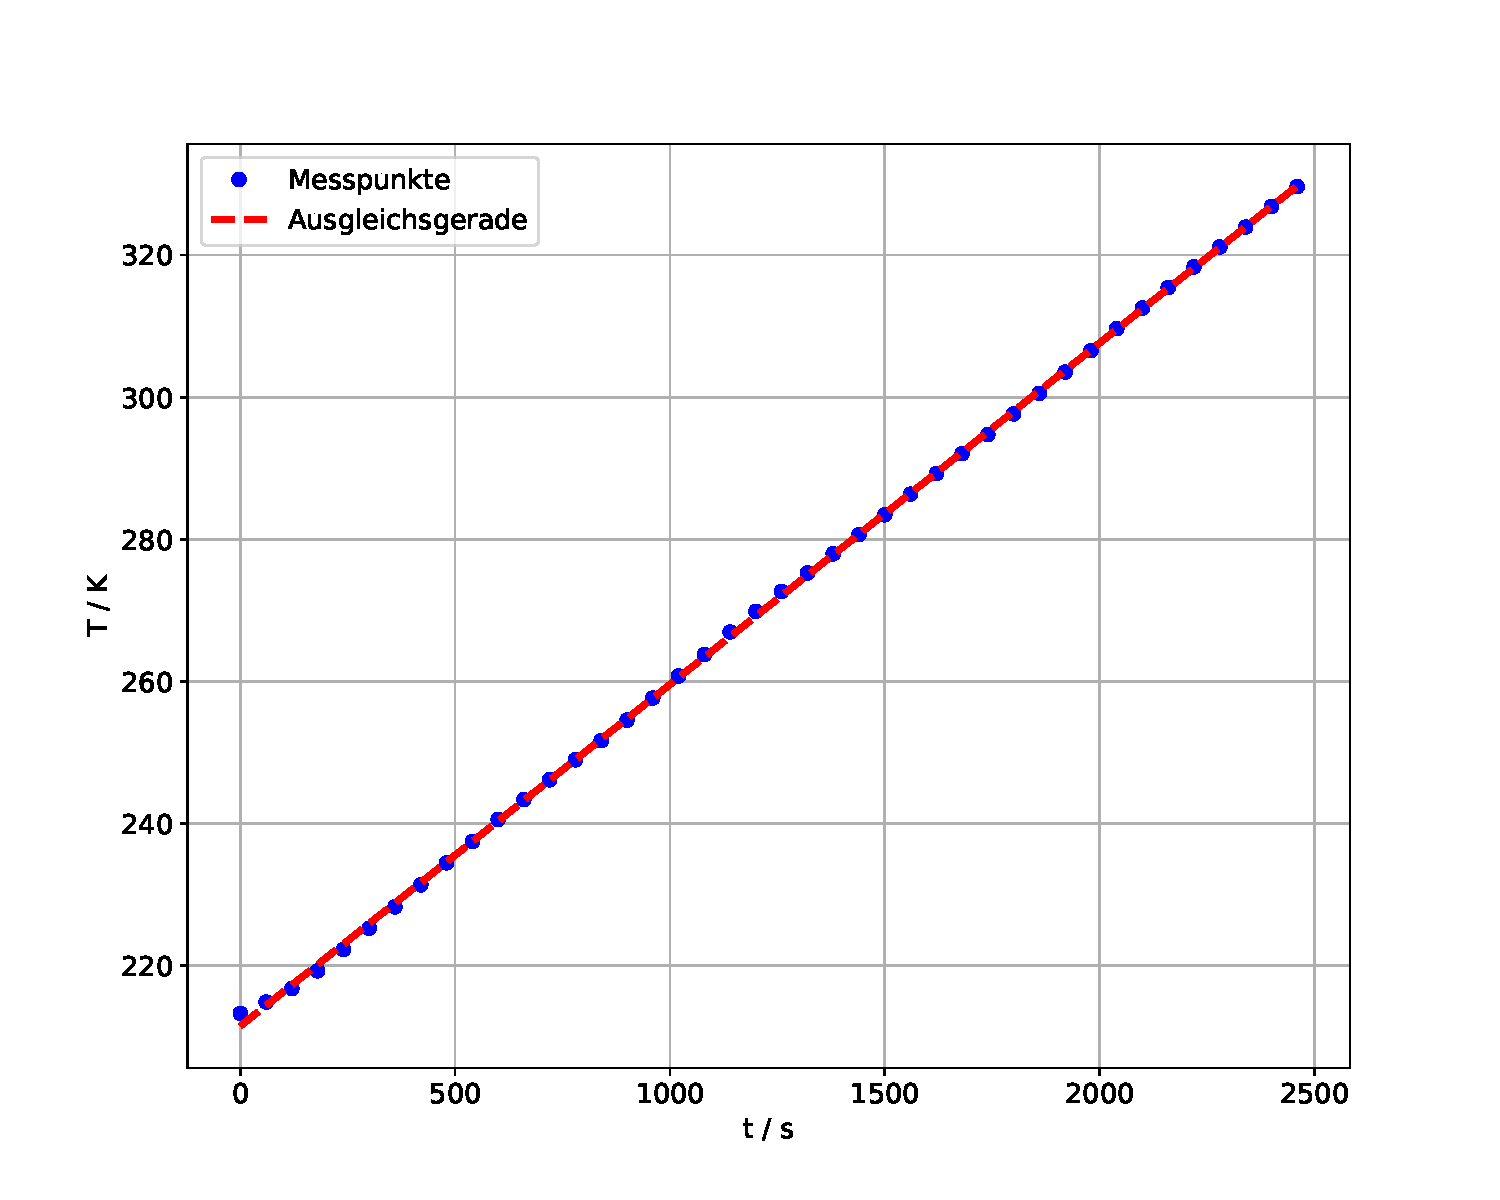
\includegraphics[width=10.0cm]{Messdaten_2_rate.pdf}
  \caption{Berechnung der mittleren Heizrate für die Messung
  mit $b_\text{heiz} \approx \SI{3.0}{\kelvin\per\minute}$}
  \label{fig:heiz2}
\end{figure}
Für die zweite Messreihe ergeben sich die Parameter
\begin{align*}
  b_\text{heiz} =& \SI{4807(10)e-05}{\kelvin\per\second} = \SI{2.884(6)}{\kelvin\per\minute}\\
  c = & \SI{211.5(1)}{\kelvin}.
\end{align*}
\subsubsection{Berechnung der der Relaxationszeit}
Die für das Berechnen der Relaxationszeit $\tau_0$ bzw. deren Fehler
notwendigen Werte sind unten dargestellt.\\
\textbf{1.Messreihe mit $b_\text{heiz} \approx \SI{1.5}{\kelvin\per\minute}$:}
\begin{align*}
  T_\text{max} =& \SI{264.25}{\kelvin} \\
  W_1 =& \SI{102(2)e-21}{\joule} \\
  b_\text{heiz} =& \SI{2434(5)e-5}{\kelvin\per\second}
\end{align*}
\textbf{2.Messreihe mit $b_\text{heiz} \approx \SI{3.0}{\kelvin\per\minute}$:}
\begin{align*}
  T_\text{max} =& \SI{263.75}{\kelvin} \\
  W_2 =& \SI{109(2)e-21}{\joule} \\
  b_\text{heiz} =& \SI{4807(10)e-5}{\kelvin\per\second}
\end{align*}
Wodurch sich durch Einsetzen in Formel \ref{eqn:tau} die Relaxationszeiten
\begin{align*}
  \tau_{0_1} =& \SI{3(2)e-10}{\second} \\
  \tau_{0_2} =& \SI{2(1)e-11}{\second}
\end{align*}
ergeben. Der Fehler berechnet sich mit Formel \ref{eqn:tau_fehler}.
% \begin{equation}
%   \Delta \tau = \sqrt{
%   \left(\frac{-\text{k}_\text{B} \, T}{W \, b^2} \cdot
%   \exp{\left(\frac{-W}{\text{k}_\text{B}  \, T}\right)} \cdot \Delta b \right)^2
%   +
%   \left(\frac{-T \, (W + \text{k}_\text{B} \, T)}{b \, W^2}
%   \cdot \exp{ \left( \frac{-W}{\text{k}_\text{B} \, T} \right)}
%   \cdot \Delta W \right)^2
%   }.
%   \label{eqn:tau_fehler}
% \end{equation}
